\chapter{Tudo ao nosso redor}
\markboth{Módulo 1}{}

%\reduline{Professor: durante a explicação inicial, não restrinja a definição do conceito de matéria, pois, nas séries seguintes, os estudantes irão se deparar com teorias mais modernas que tratam de diferentes modalidades de matéria no Universo. Ao abordar o conceito de substâncias e mistura, não se esqueça de dar exemplos; eles serão imprescindíveis para a realização das atividades. Recomenda-se que seja utilizada a lousa como suporte, tanto para a representação das moléculas em seus diferentes estados quanto para a representação dos tipos de ondas, já que são temas bastante desafiadores para os alunos devido a sua natureza não palpável. 

\section{Eixo de conhecimento do SAEB}

\begin{itemize}
  \item Matéria e energia.
\end{itemize}

\section{Habilidades da BNCC}

\begin{itemize}
  \item 
EF09CI01, EF09CI02, EF09CI03, EF09CI06.
\end{itemize}

\conteudo{O que existe em comum entre todas as coisas que compõem o universo? Tudo o
que existe é constituído de matéria (sendo a matéria tudo o que tem massa
e ocupa um lugar no espaço). Na Grécia antiga, os filósofos Leucipo e
Demócrito concluíram que a matéria pode passar por divisões sucessivas,
até alcançar uma unidade indivisível, o átomo. Ao longo do tempo, essa conclusão se
modernizou e foi complementada. Observe o esquema para verificar
o detalhamento sobre os modelos do átomo, elaborados por Dalton, Thomson, Rutherford e Bohr.

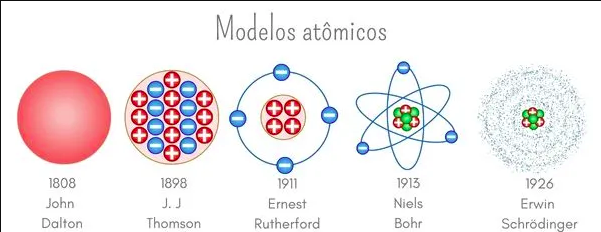
\includegraphics[width=.5\textwidth]{./imgs/img6.png}
%\caption{Fonte: https://s4.static.brasilescola.uol.com.br/be/2022/10/modelos-atomicos.jpg}

Hoje sabemos que o átomo é formando pelo núcleo (contendo prótons e
nêutrons) e pela eletrosfera (contendo elétrons). Sabemos ainda que um
conjunto de átomos com mesma propriedade constitui um elemento químico,
de forma que, em conjunto, podem formar substâncias. Essas substâncias
podem ser simples ou compostas. Juntas, duas ou mais substâncias formam
misturas, que podem ser homogêneas ou heterogêneas.

Na natureza a matéria pode ser encontrada em três estados físicos:
sólido, líquido ou gasoso. O que promove essa diferença é a organização
das moléculas, ou seja, a forma como os átomos que a compõem se organizam
e se movimentam. Há, ainda, a possibilidade de transitar entre os estados
da matéria por meio de mudanças na temperatura.

Os micro-ondas, por exemplo, são utensílios que promovem a transferência
de calor e a mudança no estado físico, por meio da agitação das moléculas
de água presentes no alimento. Isso se dá pela presença de ondas eletromagnéticas. Essas
ondas se propagam sem meios materiais, assim como o wi-fi e a luz.
Existem ainda as ondas mecânicas, que necessitam de meios materiais,
como o som. As ondas podem ser classificadas de acordo com a direção da
sua propagação (a qual pode ser uni, bi ou tridimensional) e de acordo com a direção da
vibração (a qual pode ser longitudinal ou transversal).}

\section{Atividades}

\num{1}  Leia as afirmações e marque com V as verdadeiras e com F as falsas.

\begin{boxlist}
\boxitem{F} Luz, som e calor constituídos de matéria
%\reduline{ -- Luz, som e calor são formas de energia, não de matéria}

\boxitem{V} Matéria é tudo aquilo que tem massa e ocupa lugar no espaço

\boxitem{F} A energia pode ser criada a partir da matéria
%\reduline{ -- A energia não se cria e nem se destrói, apenas se transforma}

\boxitem{F} Energia e matéria não podem sofrer transformações
%\reduline{ -- Tanto energia quanto matéria sofrem transformações}
\end{boxlist}

%\reduline{Professor, a questão avalia a capacidade do aluno de identificar afirmações falsas sobre os conceitos de matéria e energia. Atenção ao explicar o conceito de matéria, já que, para a física moderna, existem diferentes tipos de matéria no Universo.}

\num{2}  De acordo com as transformações que a matéria pode sofrer, coloque F para as transformações físicas e Q para as transformações químicas.

\begin{boxlist}
\boxitem{F} Amassar um papel

\boxitem{Q} Queimar madeira

\boxitem{F} Ferver água

\boxitem{Q} Formação de ferrugem

\boxitem{F} Misturar água com sal

\boxitem{Q} Apodrecimento do tomate
\end{boxlist}

\num{3} Escreva em ordem cronológica quais os modelos atômicos propostos pelos cientistas Dalton, Thomson, Rutherford-Bohr, apontando características principais sobre cada um deles.


\reduline{Espera-se que os alunos
descrevam o modelo de Dalton ``bola de bilhar'', descrevendo o átomo como
uma esfera maciça e indivisível; o modelo de Thomson ``pudim de passas''
e a presença de partículas subatômicas carregadas e estáticas; o modelo
de Rutherford-Bohr ``sistema solar'', que descreve o átomo como uma
estrutura formada por uma junção de partículas carregadas positivamente
no centro, chamado de núcleo e partículas com carga negativa orbitando
ao redor do núcleo formando a eletrosfera. Estimule os alunos
a pensarem sobre a evolução do conhecimento científico.\hfill}
\linhas{2}

\num{4}  Observe a imagem e indique o nome correto, o local e sua respectiva
  carga para cada uma das partes do átomo.

\begin{figure}[htpb!]

\includegraphics[width=2.02609in,height=1.43070in]{./imgs/img7.jpg}
%\caption{Fonte: Representação do átomo. Disponível em: https://pixabay.com/pt/illustrations/átomo-símbolo-personagem-resumo-68866/. Acessado em: 15 de fevereiro de 2023.}
\end{figure}

\linhas{5}

\num{5} Joana observava sua tia fazer um café e notou que, à medida que a temperatura na chaleira aumentava, mais fumaça era liberada pela própria chaleira. Joana então identificou que a molécula de água, quando exposta ao calor, muda suas características. A partir do seu conhecimento sobre moléculas e transformações físicas, avalie se a afirmação de Joana está correta e justifique.
  

\reduline{Espera-se que os alunos identifiquem que a
afirmação de Joana está correta e expliquem que o estado físico da água na chaleira muda à medida que o calor provoca agitação das moléculas de
água.\hfill}
\linhas{3}

\num{6} Dentre as misturas citadas a
  seguir, diga quais são misturas HOMOGÊNEAS e quais são HETEROGÊNEAS; no caso das
  misturas heterogêneas, cite o número de fases.

\begin{escolha}
\item
  ÁGUA + SAL: \reduline{homogênea\hfill}
\item
  ÁGUA + AREIA: \reduline{heterogênea -- duas fases\hfill}
\item
  AR ATMOSFÉRICO: \reduline{homogênea\hfill}
\item
  ÁGUA + ÓLEO: \reduline{heterogênea -- duas fases\hfill}
\item
  VINAGRE: \reduline{homogênea\hfill}
\item
  GRANITO: \reduline{heterogênea -- polifásica\hfill}
\end{escolha}

\num{7}  A energia não pode ser criada ou destruída, apenas transformada. Essa
  afirmação dá origem a imensas possibilidades de transformação no nosso
  cotidiano. Observe ao seu redor e cite pelo menos três exemplos em que
  você consegue observar transformação de energia.


\reduline{Espera-se que o aluno cite exemplos de transformação de energia
presentes no seu cotidiano, como a transformação de energia elétrica em
energia mecânica no funcionamento do ventilador, ou energia química em
energia mecânica. Professor, estimule os alunos a pensarem em
diferentes exemplos de transformação de energia em seu cotidiano, sempre
dando ênfase à conservação da energia.\hfill}
\linhas{2}

\num{8} A energia pode ter diversas fontes e inúmeras formas de ser utilizada. Pensando sobre as fontes RENOVÁVEIS e NÃO RENOVÁVEIS da energia, marque com um X as fontes de energia RENOVÁVEIS.

\begin{boxlist}
\boxitem{X} Energia Solar

\boxitem{\white{X}} Energia Nuclear

\boxitem{X} Energia Eólica

\boxitem{X} Energia Hidráulica

\boxitem{\white{X}} Energia Fóssil
\end{boxlist}

%\reduline{A questão lida com a habilidade do aluno de identificar, dentre as fontes de energia, aquelas que são renováveis, ou seja, que possuem uma fonte ilimitada e menos prejudicial ao meio ambiente durante sua obtenção e consumo. Professor, lembre-se de ressaltar que mesmo energias renováveis podem acarretar danos ambientais e que se deve sempre ter mais de uma fonte de energia para que não se sature um ambiente ou ecossistema.}

\num{9} A transmissão de imagem e a transmissão de som são essenciais para a comunicação nos
  dias atuais e, por trás dessa transmissão, existe muita física. É
  por meio do conceito de ondas que os engenheiros elaboram novas formas
  de nos comunicarmos. Sobre os tipos de ondas, marque V para verdadeiro e F para falso.

\begin{boxlist}
\boxitem{F} Ondas eletromagnéticas necessitam do meio para se propagar
%\reduline{Ondas eletromagnéticas se propagam no vácuo}

\boxitem{V} Ondas sonoras são um exemplo de ondas longitudinais 

\boxitem{F} Ondas mecânicas se propagam no vácuo
%\reduline{Ondas mecânicas necessitam do meio para se propagar}

\boxitem{V} Ondas podem ser unidimensionais, bidimensionais e tridimensionais
\end{boxlist}

\num{10} Observe a imagem e responda às questões.

\begin{figure}[htpb!]
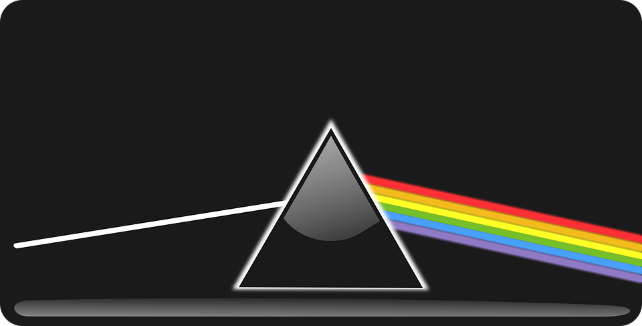
\includegraphics[width=2.91389in,height=1.47847in]{./imgs/img8.png}
\end{figure}

\begin{escolha}
\item  Que tipo de fenômeno pode ser observado na imagem?


\reduline{Refração.\hfill}
\linhas{1}

\item Que tipo de onda está relacionada com a propagação da luz?


\reduline{Ondas eletromagnéticas.\hfill}
\linhas{1}

\item Cite um exemplo em que esse conhecimento sobre a propagação da luz é utilizado no seu cotidiano.

\reduline{Câmera fotográfica, televisão, cinema etc.\hfill}
\linhas{1}
\end{escolha}

\num{11} O uso de aplicativos de mensagens foi essencial para a comunicação no período de pandemia. Com base nos seus conhecimentos de ondas eletromagnéticas, explique como é possível enviar uma imagem pelo celular para uma pessoa que se encontra em outra cidade.

%\textless{}Diagramação, por favor, baixar a imagem do banco presente no seguinte link (\url{https://pixabay.com/pt/vectors/interface-whatsapp-apps-andróide-1660652/}) e fazer o corte, deixando apenas a imagem do meio, conforme referência:

\reduline{Espera-se que os alunos descrevam que, por meio de ondas eletromagnéticas,
a mensagem enviada é transferida do emissor ao receptor, e as
frequências de onda que formam a imagem são reproduzidas no celular de
quem recebeu a foto. 
Professor, aqui é necessário se ater apenas ao
conceito básico de transmissão de informação por ondas eletromagnéticas,
em especifico a transmissão de imagem, já que esse processo é muito mais
complexo do que o conjunto de conhecimentos trabalhados até aqui. Pode
ser sugerido que os alunos pesquisem em casa sobre esse processo e sobre como
funciona a tecnologia Wi-Fi.\hfill}

\section{Treino}

\num{1}

\begin{quote}
``A The Ocean Cleanup é uma ONG que pretende acabar com a Grande
Mancha do Pacífico, a imensa ilha de plástico que flutua no maior dos
oceanos, usando um sistema que captura o lixo, que depois será retirado por um navio. 
O sistema funciona com uma grande barreira
flutuante e uma tela que fica submersa a uma profundidade de 3 metros, e pode capturar o lixo que não está boiando na superfície. [...]''

\fonte{Nick Ellis. MeioBit. The Ocean Cleanup: sistema de barreiras flutuantes quer tirar plástico
do Pacífico. Disponível em:
https://meiobit.com/390064/the-cleanup-ocean-limpar-plastico-do-pacifico/.
Acesso em: 17 fev. 2023.}
\end{quote}

A ideia de catar o lixo boiando sobre a água que será barrada pelas barreiras desenvolvidas pela ONG só é possível graças a que propriedade da matéria?

\begin{escolha}
\item Volume.

\item Maleabilidade.

\item Brilho.

\item Densidade.
\end{escolha}

\num{2}

\begin{quote}
Pesquisadores descrevem movimento de elétrons que levam à aurora
pulsante, evento multicolorido e brilhante na magnetosfera. O que os
cientistas conseguiram observar foi uma evidência direta da origem da
aurora pulsante: uma verdadeira chuva de elétrons envolvida em ondas
de plasma (estado físico da matéria similar ao gás, mas com partículas
ionizadas).

\fonte{Adaptado de G1. Cientistas observam 'chuva de elétrons' que dá origem a
fenômeno brilhante no céu. 
Disponível em:
https://g1.globo.com/ciencia-e-saude/noticia/cientistas-observam-chuva-de-eletrons-que-da-origem-a-fenomeno-brilhante-no-ceu-veja-video.ghtml.
Acesso em: 19 fev. 2023.}
\end{quote}

Quais características do elétron fazem com que eventos como a aurora
pulsante seja possível?

\begin{escolha}
\item
  Elétrons encontram-se no núcleo do átomo e liberam energia mudando entre as camadas de valência.
\item
  Elétrons são partículas neutras que transferem cargas elétricas ao se movimentarem pela eletrosfera.
\item
  Elétrons são partículas de carga negativa que se encontram na eletrosfera, capazes de se movimentar liberando energia.
\item
  Elétrons possuem cargas negativas, presas ao núcleo, que, quando se movimentam, liberam energia.
\end{escolha}


\num{3}

\begin{quote}  
Você tem a sensação de que o sinal de Wi-Fi fica mais fraco no
banheiro do que em outros cômodos? Saiba que isso não é um mito e
existe uma explicação para isso. Os grandes vilões do Wi-Fi no
banheiro são os espelhos. Quanto maior seu tamanho, maior é a chance
de ele interferir no sinal da Internet. Isso porque, por trás do
vidro, há uma camada de metal, responsável por refletir a luz.

\fonte{Entenda por que o sinal da Internet Wi-Fi é mais lento no banheiro. G1
Techtudo. 03/11/2018. Disponível em:
https://www.techtudo.com.br/listas/2018/11/entenda-por-que-o-sinal-da-internet-wi-fi-e-mais-lento-no-banheiro.ghtml.
Acesso em: 19 de fevereiro de 2023.}
\end{quote}

Com base nas informações do texto e em seus conhecimentos, justifique a
relação da presença de espelhos no banheiro com a baixa qualidade de
sinal de Wi-Fi nesse ambiente.

\begin{escolha}
\item
  O sinal do Wi-Fi é transmitido através de ondas eletromagnéticas que
  são capturadas pelo metal que é bom condutor de energia, atrapalhando
  a transmissão.
\item
  A transmissão Wi-Fi acontece por meio de ondas mecânicas; dessa forma,
  estruturas sólidas com potencial de reflexão, como os espelhos,
  atrapalham a transmissão.
\item
  A camada de metal reflete sinal de Wi-Fi, evitando que ele se
  propague, já que se trata de ondas eletromagnéticas, que necessitam de
  objetos para se propagar no meio.
\item
  O sinal do Wi-Fi é transmitido com base nos mesmos princípios que o som
  e sua propagação depende de meios opacos para acontecer; o brilho do
  espelho dificulta a transmissão.
\end{escolha}


\chapter{Evoluir}
\markboth{Módulo 2}{}

%\reduline{Professor: durante a explicação das teorias evolucionistas, recomendamos que você utilize a lousa como recurso para deixar claras as ideias antagonicas existentes nas teorias de Lamarck e Darwin. Além disso, é importante ressaltar que as ideias de Lamarck, apesar de não aplicadas hoje, foram importantes para que estudiosos da época pudessem basear seus estudos; assim você mostra aos alunos que a ciência é construída ``de passo em passo'' e em conjunto. Durante a explicação sobre classificação biológica, lembre-se de ressaltar que REINO é a categoria mais abrangente, enquanto ESPÉCIE é a categoria mais específica. Também é importante comentar que os nomes costumam estar em latim e que o nome da espécie e do gênero devem estar destacados. Para finalizar a aula, converse com os estudantes sobre a diversidade de espécies presentes em nosso país e proponha que, em grupos, elaborem propostas de intervenção que possam conter o avanço do desmatamento em nosso país.


\section{Eixo de conhecimento do SAEB}
\begin{itemize}
  \item Vida e evolução.
\end{itemize}

\section{Habilidades da BNCC}

\begin{itemize}
  \item 
EF09CI08, EF09CI10, EF09CI12.
\end{itemize}

\conteudo{Hoje conhecemos cerca de 1,5 milhão de espécies presentes em nosso
planeta. Mas as estimativas vão além, dizem que existem de 10 a 50
milhões de seres vivos que ainda não foram classificados! Cada uma
dessas espécies possui características individuais e modo singular de
interagir com o meio biótico (conjunto de seres vivos, como fauna e
flora) e abiótico (conjunto de seres não vivos, como água e luz). Mas
como pode haver uma diversidade tão imensa de seres vivos?

Há muito tempo, estudiosos se fizeram essa mesma pergunta e, a partir dela,
começaram a cunhar as teorias evolucionistas, que afirmam que os seres
vivos mudam ao longo do tempo. Lamarck acreditava que os seres vivos
mudariam para se adaptar em um ambiente e essas novas características
adquiridas seriam repassadas. Já Darwin afirmou que as mudanças
existentes entre as espécies eram decorrentes da seleção natural, ou
seja, os seres vivos mais aptos seriam selecionados pelo ambiente;
sobrevivendo, poderiam se reproduzir e repassar seus caracteres.

Hoje
sabemos que a evolução das espécies é um processo constante, atemporal, que
acontece há milhões de anos e atua sobre todos os organismos vivos
selecionando as espécies que se adaptam às mudanças ambientais. Diante
disso, surge outra questão: como organizar tantos seres? Na
biologia, temos organizações hierárquicas, por meio das quais podemos organizar a
vida desde átomos, passando por células e sistemas, até ecossistemas e a própria biosfera, conforme a figura.


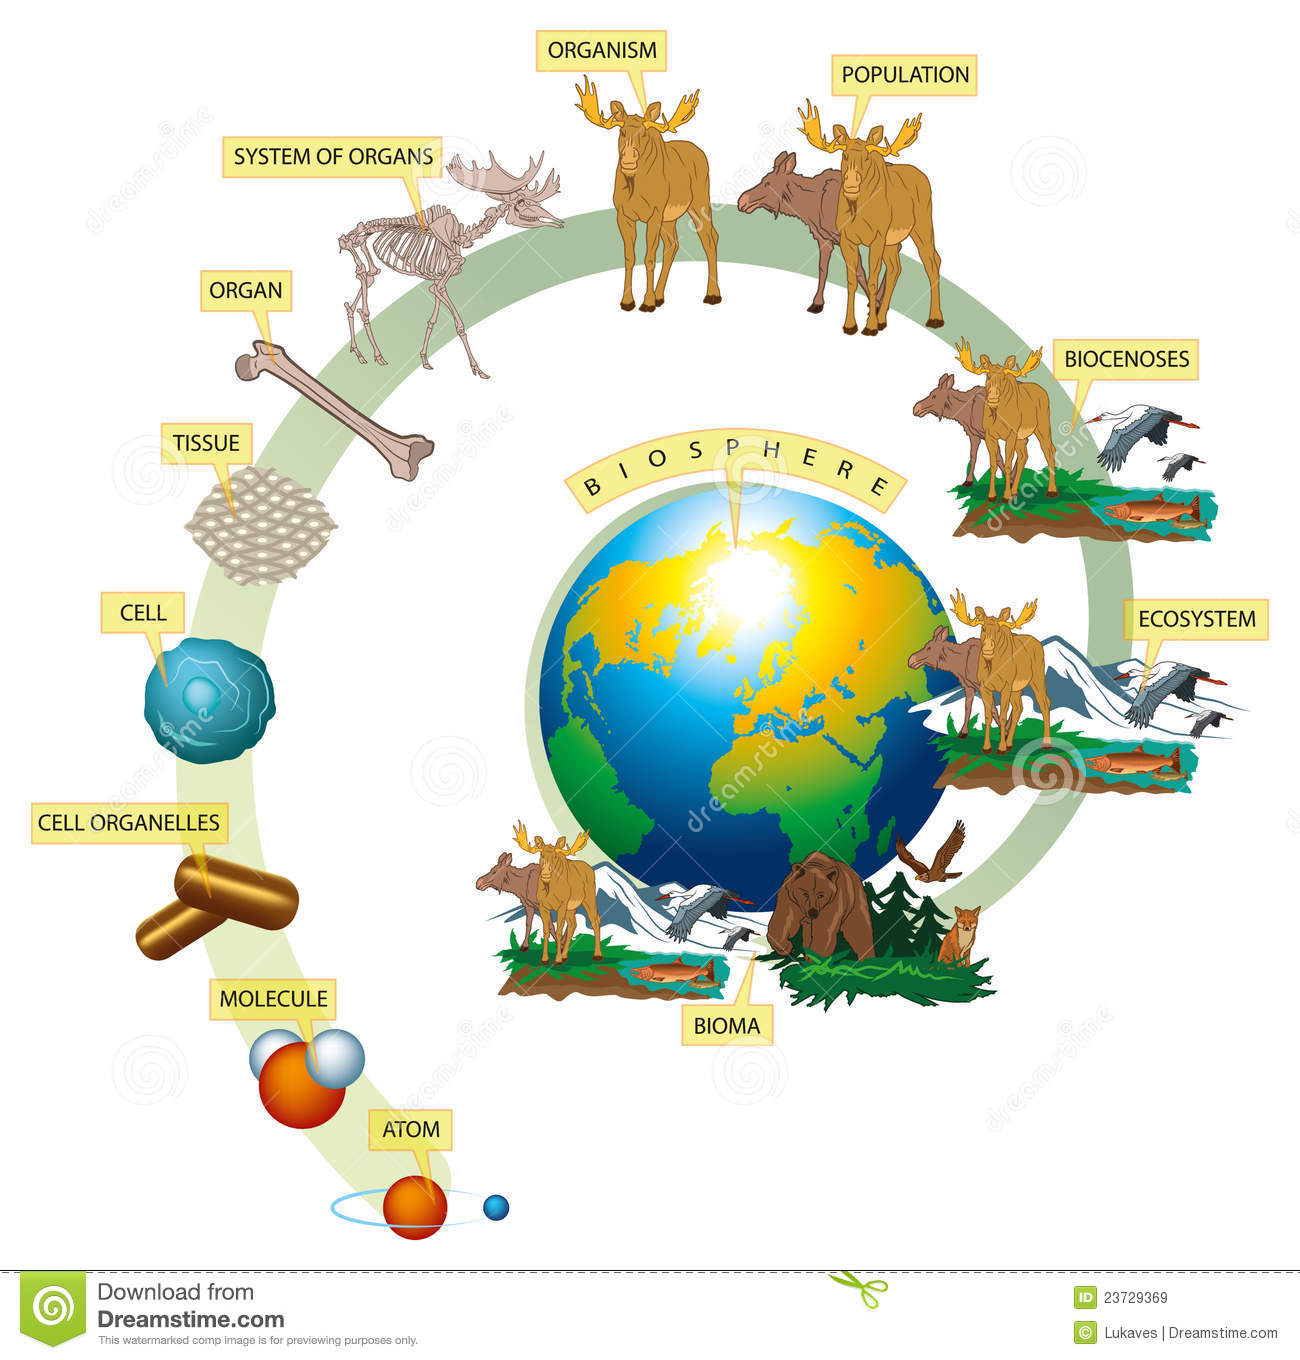
\includegraphics[width=1.71875in,height=1.66389in]{./imgs/img9.jpg}
%\caption{Fonte: https://www.dreamstime.com/royalty-free-stock-images-living-world-image23729369}

Ou podemos seguir de uma maneira mais específica, organizando as
espécies que existem no planeta por meio da classificação biológica.
Essa tarefa é tão extensa que existe uma área específica dedicada a
identificar, nomear e classificar os seres vivos: a taxonomia. Veja a
seguir os níveis taxonômicos de organização da espécie humana.

Nossa espécie é uma das que mais se prolifera no mundo, ao passo que
também é uma das que mais o destrói. O Brasil, por exemplo, tem seis biomas: Amazônia, Caatinga, Cerrado, Pantanal, Mata Atlântica e Pampa. Todos
já têm uma porcentagem destruída, sendo o desmatamento da Amazônia um
dos mais graves. Além do desequilíbrio ambiental provocado pela perda da
vegetação nativa, há ainda a problemática do aumento da transmissão de
doenças, tendo em vista que animais silvestres perdem seu habitat e
passam a viver mais próximos da população humana, podendo disseminar
doenças. Um exemplo é a COVID-19. Acredita-se que a zoonose estava
presente em morcegos e acabou alcançando a espécie humana devido à caça
desses animais. Portanto, é evidente que tanto o meio ambiente depende
de nós quanto nós dependemos dele para coexistirmos. E, como ferramenta
aliada nesse processo de conservação das espécies, vale destacar as
unidades de conservação.}

\section{Atividades}

\num{1} Jean-Baptiste de Lamarck foi um naturalista, assim como Charles
  Darwin. Ambos se interessaram por um mesmo processo: a evolução das
  espécies. A partir de suas observações, cada um deles elaborou teorias
  que explicassem esse processo. Sabendo disso, responda:

\begin{escolha}
\item Em que consiste a teoria de cada um deles?

\reduline{Lamarck acreditava que os seres vivos poderiam mudar espontaneamente
para se adaptar ao ambiente; girafas, por exemplo, ao fortalecer o
pescoço, poderiam acabar fazendo-o crescer e, ao se reproduzir, passariam
essa características a seus descendentes. Darwin acreditava que os seres
vivos mais aptos a um determinado ambiente passariam por um processo de
seleção natural. Girafas de pescoço mais longo, por exemplo, seriam
privilegiadas por conseguirem se alimentar mais facilmente e
sobreviveriam no ambiente, enquanto as de pescoço curto enfretariam mais
desafios para conseguir se alimentar e poderiam acabar morrendo sem passar seus genes adiante.\hfill}

\item Apesar das diferenças, as teorias desses dois estudiosos tinham pontos em comum. Quais eram?

\reduline{Ambos acreditavam que as espécies se modificavam com o tempo, que as
características eram passadas para seus descendentes e que essas
características eram influenciadas de alguma forma pelo ambiente.\hfill}
\end{escolha}

\num{2}

\begin{quote}
Quando se fala em biodiversidade, costuma-se pensar no verde das florestas. Mas é no azul dos oceanos que está a última fronteira da vida e a maior diversidade de espécies do planeta. [...] Por exemplo, robôs a serviço do censo descobriram sob o gelo do Ártico uma cadeia vulcânica coberta por micro-organismos. Um satélite localizou uma aglomeração de centenas de tubarões no meio do Pacífico Norte. Fontes quentes em águas gélidas são o lar de peixes bizarros e vermes gigantes. Até a década passada, o homem conhecia cerca de 230 mil espécies marinhas. Esse contingente saltou para quase 236 mil. E estima-se que o número real ultrapasse um milhão, pelo menos. Juntos, os 17 projetos do Censo exploraram 5\% dos oceanos. [...]

\fonte{Renato Grandelle. O Globo. Oceanos abrigam a maior diversidade da Terra. Disponível em: 
https://oglobo.globo.com/saude/ciencia/oceanos-abrigam-maior-diversidade-da-terra-3036406.
Acesso em: 23 fev. 2023.}
\end{quote}

O que explica a grande diversidade encontrada por esses pesquisadores
durante sua exploração no oceano?


\reduline{Tendo em vista que o oceano é um ambiente extenso e diverso, pode-se
afirmar que, ao longo da evolução das espécies marinhas, elas foram
selecionadas para conseguir sobreviver em cada um desses ambientes, o
que gerou a alta diversidade de espécies existentes no oceano.\hfill}
\linhas{2}

\num{3}

\begin{quote}
O exemplo clássico da hipótese de Lamarck é o das girafas, que depois ficou conhecida como "lamarquismo": os animais teriam herdado o pescoço longo de seus antepassados, e essa característica foi se aprofundando para permitir alcançar os ramos mais altos das árvores, de cujas folhas elas se alimentam.

Mas em 1859, a hipótese de Lamarck foi ofuscada quando Charles Darwin
lançou o livro A Origem das Espécies. Na obra, o britânico descreve como
os traços de cada espécie viva surgem ao longo de várias gerações,
conforme mutações genéticas benéficas são selecionadas pelo ambiente.
Hoje, a teoria da Evolução de Charles Darwin é considerada um fato
científico.

\fonte{Fonte de pesquisa: BBC Brasil. Como uma aldeia no Ártico ajudou a ampliarmos o que sabemos
sobre Evolução. Disponível em: \textit{https://www.bbc.com/portuguese/geral-42420424}.
Acesso em: 23 fev. 2023.}
\end{quote}

Apesar da ideia de Lamarck não ser aplicada hoje, ela foi importante
para os estudiosos da época. Explique o porquê.


\reduline{Lamarck teve ideias revolucionárias para seu tempo ao refletir sobre a
influência do meio ambiente sobre os organismos. Apesar de não ter
formulado a teoria que utilizamos hoje (evolução por meio da seleção
natural), suas ideias estabeleceram as bases para que, posteriormente,
estudiosos pudessem refletir mais sobre o cenário exposto por ele e
elaborar o conceito que adotamos hoje.\hfill}
\linhas{3}

\num{4}  Sobre os níveis de organização em biologia, marque V para verdadeiro ou F para falso.

\begin{boxlist}
\boxitem{(V)} A organização começa no átomo.

\boxitem{(V)} A célula é a unidade básica da vida.

\boxitem{(F)} O nível mais alto e complexo é o organismo.

\boxitem{(F)} Um conjunto de ecossistemas forma uma comunidade.
\end{boxlist}

\num{5}  O corpo humano é muito complexo, formado por \reduline{sistemas} 
  que trabalham em conjunto para que o organismo funcione o melhor possível e para que a sobrevivência do indivíduo se garanta.

\fonte{Fonte de pesquisa: Jornal da USP. Físicos investigam interações.
https://jornal.usp.br/ciencias/ciencias-exatas-e-da-terra/fisicos-investigam-interacoes-entre-sistemas-do-corpo/
. Acesso em 23/02/2023.}

Qual nível de organização biológica melhor preenche a lacuna do texto?
Cite alguns exemplos do agrupamento citado.

\reduline{Sistemas. Sistema respiratório, nervoso, esquelético, reprodutor.\hfill}
\linhas{1}

\num{6}  Escreva, em ordem hierárquica, os níveis de organização biológica existentes.

\reduline{Átomo, mólecula, organela, célula, tecido, órgão, sistema, organismo,
população, comunidade, ecossistema, bioma, biosfera.\hfill}
\linhas{2}

\num{7}

\begin{quote}
\textbf{Seres vivos ganham nova classificação após 285 anos.}

O universo científico criou uma nova forma de classificar os organismos
vivos 285 anos após a invenção do Systema Naturae pelo botânico sueco
Carlos Lineu. A nova proposta, publicada nos livros PhyloCode e
Phylonym, leva em consideração a Teoria da Evolução de Charles Darwin e
foi organizada por cerca de 200 especialistas. 
Entre os responsáveis
pela nova classificação, o professor Max Cardoso Langer, do Departamento
de Biologia, da Faculdade de Filosofia, Ciências e Letras de Ribeirão
Preto (FFCLRP) da USP, explica que a modificação foi necessária porque a
invenção de Lineu é anterior à teoria de Darwin e, naquela época,
classificou os organismos pelas características anatômicas. Lineu não
sabia que ``os organismos mudam morfologicamente ao longo do tempo'',
mas, apesar disso, ``o sistema de denominação permanece sendo como o
daquela época''.  [...]
Para o novo sistema, cientistas buscaram por linhagens
evolutivas dos seres para então defini-los. ``Ao invés de definir as
aves como os animais que têm penas, podemos definir, por exemplo,
colocando todas as aves viventes em uma árvore filogenética e descer a
linha de ancestralidade até chegar a um único ancestral comum. Todas as
espécies que descendem desse ancestral comum serão chamadas aves.'' [...]

\fonte{Tainá Lourenço. Jornal da USP. Seres vivos ganham nova classificação após 285 anos. Disponível em: 
https://jornal.usp.br/ciencias/seres-vivos-ganham-nova-classificacao-apos-285-anos/
. Acesso em: 23 fev. 2023.}
\end{quote}

A qual área da biologia o texto está se referindo?


\reduline{Taxonomia, ramo responsável por descrever, identificar e nomear os seres
vivos de acordo com critérios de classificação.\hfill}
\linhas{2}

\num{8}  Acerca do padrão de nomenclatura biológica das espécies, marque V para verdadeiro ou F para falso.

\begin{boxlist}
\boxitem{F} homo sapiens é a forma correta de escrita do nome da espécie humana.

\boxitem{V} A nomeclatura científica é, obrigatoriamente, binomial.

\boxitem{F} O primeiro nome é chamado de epíteto específico e o segundo de
epíteto genérico.

\boxitem{F} O latim foi escolhido para nomear espécies por ser uma língua bonita
e culta.

\boxitem{V} \emph{Trichechus manatus} e \emph{Trichechus inunguis} são duas
espécies pertencentes a um mesmo gênero.

\boxitem{V} As regras de nomeclatura científica permitem que cientistas de
qualquer local do mundo possam compartilhar informações sobre as
espécies existentes.
\end{boxlist}

\num{9}  A seguir você encontra todas as categorias taxonômicas existentes.

\begin{myquote}
GÊNERO -- CLASSE -- FILO -- ESPÉCIE -- FAMÍLIA -- ORDEM -- REINO
\end{myquote}

Ordene-as de maneira hierárquica, da mais abrangente à mais específica.


\reduline{Reino -- Filo -- Classe -- Ordem -- Família -- Gênero -- Espécie\hfill}
\linhas{2}

\num{10}  Sobre as categorias taxonômicas, marque V para verdadeiro ou F para falso.

\begin{boxlist}
\boxitem{F} Família é a categoria mais abrangente.

\boxitem{V} Espécie é a categoria mais específica.

\boxitem{V} Ornitorrincos e seres humanos, apesar de bem diferentes, ocupam a
mesma classe por serem mamíferos.

\boxitem{F} Existem seis reinos distintos: animalia, plantae, fungi, monera,
protista e vírus.
\end{boxlist}

\num{11} Trata-se de um bioma exclusivamente brasileiro, responsável por abrigar o Semiárido. 
  Ocupa cerca de 11\% do território do Brasil, além de 54\% do da Região
  Nordeste. Paulo
  Pedro de Carvalho, representante do Centro de Assessoria e Apoio aos
  Trabalhadores e Instituições Não Governamentais Alternativas, afirmou foi o bioma que mais sofreu
  degradação em consequência de mudanças climáticas.

\fonte{Fonte de pesquisa: Agência Senado. Disponível em:
https://www12.senado.leg.br/noticias/materias/2022/04/27/audiencia-destaca-riqueza-da-caatinga-e-alerta-para-efeitos-das-mudancas-climaticas-no-bioma
. Acesso em: 23 fev. 2023.}

\begin{escolha}
\item A que bioma o texto se refere?


\reduline{Caatinga\hfill}
\linhas{1}

\item Quais os outros biomas que o nosso país abriga?


\reduline{Cerrado, Pampa, Mata Atlântica, Amazônia, Pantanal.\hfill}
\linhas{1}
\end{escolha}

\num{12}  Sobre conservação da biodiversidade, marque V para verdadeiro ou F para falso.

\begin{boxlist}
\boxitem{V} Unidade de conservação é uma área que engloba tanto espaço
territorial quanto recursos naturais, tendo como objetivo a conservação
da fauna e da flora de uma região.

\boxitem{F} A contaminação da água, do solo e do ar, assim como a destruição de
habitat e o uso sustentável de recursos são ameaças para a
biodiversidade. 

\boxitem{V} As unidades de conservação de proteção integral têm como objetivo
manter a natureza livre da interferência humana, enquanto a de uso
sustentável preza pela conciliação entre conservação e uso sustentável
de recursos.

\boxitem{V} Biodiversidade é um termo que descreve a riqueza de espécies
existentes no planeta, incluindo plantas, animais, fungos e
microorganismos. A conservação e a sobrevivência desses seres está
intimamente ligada à sobreviência da espécie humana.
\end{boxlist}


\section{Treino}

\num{1}

\begin{quote}
Mais de 21 anos após o anúncio do descobrimento da sequência genética
  dos humanos, a coalizão do Projeto do Genoma Humano publicou um artigo
  científico que estabelece o primeiro mapa genético totalmente completo
  da espécie humana. 
  Até 2021, cerca de 92\% do código genético humano
  era conhecido. Segundo os autores do estudo, publicado na revista
  científica Science, as novas informações trazem dados importantes
  sobre doenças e características evolutivas da raça humana. [...]

\fonte{Agência Brasil. Cientistas publicam artigo que conclui mapeamento ge^nético humano. Disponível em: https://agenciabrasil.ebc.com.br/saude/noticia/2022-03/cientistas-publicam-artigo-que-conclui-mapeamento-genetico-humano. Acesso em: 23 fev. 2023.}
\end{quote}

A investigação das características citadas é possível graças à

\begin{escolha}
\item
  Hereditariedade.
\item
  Paleontologia.
\item
  Conservação.
\item
  Taxonomia.
\end{escolha}

\num{2}

\begin{quote}
Em um estudo recente, cientistas da França e daEspanha estudaram a
  coloração ornamental da ave chapim-azul (\emph{Cyanistes caeruleus}).
 Essa ave caracteriza-se por apresentar coloração vistosa, com coroa azul e peito amarelo.
Segundo os estudos, em duas populações estudadas, as coroas azuis e os peitos amarelos
  são menos visíveis do que quando o estudo começou. Ademais, em épocas mais quentes e secas, as aves apresentavam também cores menos
  vivas. Isso, juntamente com o aumento da
  temperatura e a diminuição da precipitação na área de estudo, sugere que
  a redução da coloração nessa população é consequência das mudanças climáticas.

\fonte{Fonte de pesquisa: David López Idiáquez. BBC Brasil. Por que os pássaros estão perdendo suas cores. Disponível em: https://www.bbc.com/portuguese/geral-62048972. 
Acesso em: 23 fev. 2023.}
\end{quote}

Qual teoria explica o fenômeno apresentado na pesquisa?

\begin{escolha}
\item
  Seleção natural: ao notar as mudanças ambientais, os pássaros se
  modificaram para que pudessem sobreviver.
\item
  Lamarckismo: ao notar as mudanças ambientais, os pássaros se
  modificaram para que pudessem sobreviver.
\item
  Seleção natural: a mudança ambiental exerce uma pressão sobre a
  espécie, selecionando apenas os mais aptos à sobrevivência.
\item
  Lamarckismo: a mudança ambiental exerce uma pressão sobre a espécie,
  selecionando apenas os mais aptos à sobrevivência.
\end{escolha}

\num{3}

\begin{quote}
\textbf{Idema propõe criação de nova unidade de conservação da caatinga no Rio
Grande do Norte}

"Refúgio da Vida Silvestre" será área de proteção do bioma e de
preservação das cabeceiras da bacia hidrográfica do Rio Potengi, segundo
órgão.

O Instituto de Desenvolvimento Sustentável e Meio Ambiente (Idema)
propôs a reserva de uma área para criação de uma unidade de conservação
da caatinga e das cabeceiras da bacia hidrográfica do Rio Potengi, no
Rio Grande do Norte. [...]

\fonte{G1. Idema propõe criação de nova unidade de conservação da caatinga no Rio
Grande do Norte. Disponível em:
https://g1.globo.com/rn/rio-grande-do-norte/noticia/2022/11/26/idema-propoe-criacao-de-nova-unidade-de-conservacao-da-caatinga-no-rio-grande-do-norte.ghtml
. Acesso em: 23 fev. 2023.}
\end{quote}

Qual alternativa indica uma possível justificativa para defender a criação da unidade de conservação citada?

\begin{escolha}
\item
  Devido à baixa riqueza de espécies na Caatinga, é necessário que haja
  normas garantindo o isolamento geográfico desses indivíduos.
\item
  Devido à alta diversidade biológica endêmica e à extensão da Caatinga,
  é necessário que haja normas garantindo a proteção adequada.
\item
  Devido à alta diversidade biológica e à extensão da Caatinga, é
  necessário criar medidas que favoreçam o comércio das espécies exóticas da região.
\item
  Devido à baixa riqueza de espécies na Caatinga, é necessário que haja
  incentivos para a criação de indústrias na área.
\end{escolha}

\chapter{Onde vivemos}
\markboth{Módulo 3}{}

%\reduline{Professor, durante a explicação acerca do surgimento do universo, ressalte que o movimento da matéria não ocorreu somente no momento do Big Bang. Reforce que o universo está em constante expansão e, portanto, as galáxias estão se afastando. Se achar pertinente, durante a explicação sobre o sistema solar, aprofunde-se nas características individuais de cada planeta, comentando, por exemplo, sobre os anéis de Saturno. Para falar sobre a Terra, procure vincular suas características ao dia a dia dos estudantes.  Para isso você pode perguntar como os fenômenos comentados os impactam e qual a importância da translação, por exemplo, para o cotidiano deles.

\section{Eixo de conhecimento do SAEB}
\begin{itemize}
  \item Terra e universo.
\end{itemize}

\section{Habilidades da BNCC}

\begin{itemize}
  \item 
EF09CI14, EF09CI16, EF09CI17.
\end{itemize}

\conteudo{De onde viemos? 
Para responder a essa pergunta temos de voltar bilhões de anos, quando
toda a matéria e energia estavam contidas em um único ponto, até que um
desequilíbrio provocou uma grande explosão chamada de ``Big Bang''.
Nesse segundo, toda a matéria se estendeu ao longo do espaço infinito.
Ao contrário do que se pode pensar, esse processo de expansão continua e
continuará aumentando. Mas cientistas já levantaram a hipótese de uma
contração final, que fará tudo retornar ao ponto inicial. Esse movimento
foi chamado de ``Big Crunch''.

Mas, afinal, onde estamos em meio a essa estrutura em expansão? Dentre as
milhares de galáxias existentes, fazemos parte da Via Láctea. Nela,
diversas estrelas nascem e morrem constantemente. E nós estamos em um
sistema ao redor da estrela a que chamamos de Sol. Nesse sistema estão
incluídos oito planetas: Mercúrio, Vênus, Terra e Marte (Esses planetas
são formados principalmente por rochas, por isso são chamados de
terrestres ou telúricos); Júpiter, Saturno, Urano e Netuno (Esses
planetas são formados principalmente por gases, por isso são chamados de
gasosos ou jovianos). Além deles, há ainda diversos satélites naturais
(como a nossa Lua), cometas, asteroides e outras partículas que vagam
por nossa galáxia. Por fim, é importante saber que Plutão (conhecido
como ``planeta anão'') é um corpo celeste presente em nosso sistema
solar que, devido a uma decisão da União Astronômica Internacional, deixou
de ser considerado planeta. O principal motivo dessa decisão foi o fato de Plutão
não ter massa suficiente para limpar sua órbita de objetos menores.
Existem outros planetas anões como ele: Ceres, Haumea, Makemake e Éris.

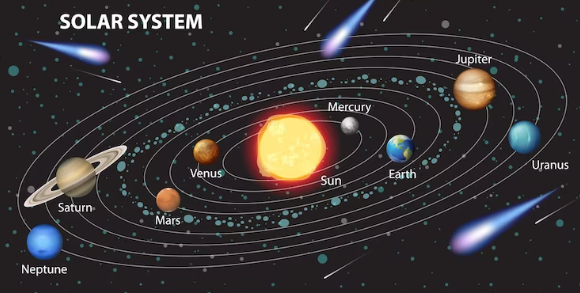
\includegraphics[width=1.78261in,height=0.90032in]{./imgs/img10.png}
%\caption{Fonte: https://br.freepik.com/vetores-gratis/sistema-solar-para-o-ensino-de-ciencias_24085043.htm\#query=sistema\%20solar\&position=5\&from_view=search\&track=ais}

Todos os planetas possuem dois movimentos: rotação (em torno do seu
próprio eixo) e translação (em torno do Sol). Vale ressaltar que
satélites, como a Lua, também se movimentam. A Lua gira em torno de si
mesma (rotação) e em torno da Terra (revolução). Em conjunto esses
movimentos dão origem às fases lunares. Especificamente sobre a Terra, a
rotação dura cerca de 24 horas. Ao longo desse período uma parte no
planeta fica iluminada pelo sol, enquanto a outra fica escura,
originando assim os dias e as noites. Já a translação dura cerca de 365
dias, 5 horas, 48 minutos e 48 segundos; esse movimento está ligado ao fenômeno das estações do ano.

Além dessas características, a Terra tem um outro atributo que a torna
especial dentre os planetas do nosso sistema solar: a vida. A
temperatura amena, a atmosfera contendo oxigênio e a presença da água em
forma líquida são fatores que favoreceram o aparecimento da vida no
planeta. Os organismos vivos habitam a camada mais superficial da Terra,
chamada de crosta, formada por rochas, minerais e solo. Entretanto,
nessa região enfrentamos diversos problemas ambientais, como
desmatamento, poluição das águas e do ar, degradação do solo e muitos
outros. Todos esses, em conjunto, têm levado à extinção de diversas
espécies. Além da crosta, a Terra é formada também pelos mantos superior e
inferior, por camadas intermediárias e pelo núcleo, camada mais interna.}

\section{Atividades}

\num{1}  Trienalmente, a União Astronômica Internacional se reúne para tomada
  de decisões sobre astronomia e todas as suas vertentes. Em 2006,
  formularam uma nova classificação para os corpos celestes do Sistema
  Solar, na qual Plutão deixou de ser considerado planeta. Explique a
  principal característica que levou o grupo a tomar essa decisão.


\reduline{Para que um corpo celeste seja considerado planeta ele deve ser capaz de
apresentar uma órbita própria, e Plutão não atendia a esse requisito,
tendo sua órbita dependente de outros corpos celestes.\hfill}
\linhas{2}

\num{2} Os planetas do Sistema Solar podem ser classificados de acordo com sua
  composição. Sabendo disso, marque V para as afirmações verdadeiras e F para as falsas.

\begin{boxlist}
\boxitem{F} Marte é um planeta Joviano devido a sua composição rochosa.

\boxitem{V} Saturno é um planeta composto por hidrogênio, hélio e metano;
portanto, pode-se afirmar que é um planeta gasoso.

\boxitem{F} A Terra é um planeta Joviano devido ao surgimento tardio de vida em
sua crosta.

\boxitem{V} Assim como Mercúrio, Vênus é um planeta Telúrico.
\end{boxlist}

\num{3}  Complete as lacunas a seguir.

\reduline{Mercúrio} é um planeta rochoso, conhecido por ser
o mais próximo do Sol e, portanto, o primeiro do nosso sistema solar. Em
contrapartida, \reduline{Netuno} é um planeta gasoso e o mais distante
do Sol; devido a essa característica, suas temperaturas são muito
baixas, podendo alcançar -200°C. 

\num{4}  Em nosso sistema solar, existem cinco planetas classificados como anões. Cite o nome de cada um deles.


\reduline{Plutão, Ceres, Haumea, Makemake, Eris.\hfill}
\linhas{1}

\num{5}  Sobre os movimentos do planeta Terra, marque R para características da rotação e T para características da translação.

\begin{boxlist}
\boxitem{R} Dura 24 horas.

\boxitem{T} Origina as estações do ano.

\boxitem{T} Dura 365 dias e alguns minutos, o que gera, após 4 anos, um ano
bissexto.

\boxitem{R} Origina os dias e as noites.
\end{boxlist}

\num{6}  O que é o Big Bang? Explique como e quando esse fenômeno ocorreu.


\reduline{O Big Bang foi uma grande explosão gerada pelo acúmulo de energia e
calor em um ``átomo primordial'' extremamente denso. Após a explosão
toda a matéria entrou em expansão e assim se encontra até hoje.\hfill}
\linhas{1}

\num{7}

\begin{quote}
Era uma teoria, já descartada, segundo a qual o Universo se contrairia até
  se reduzir a um único ponto, denso e quente, e então entraria em
  colapso -- quase como o inverso do Big Bang. Cientistas acreditavam
  que isso aconteceria porque a atração gravitacional poderia diminuir a
  velocidade de expansão das galáxias. Mas a hipótese foi derrubada em
  1998. ``Hoje sabemos que a densidade do Universo é baixa demais e que
  sua expansão não está desacelerando, e sim aumentando'', explica Raul
  Abramo, do Instituto de Física da USP. [...]

\fonte{Giselle Hirata. Superinteressante. Disponível em: 
https://super.abril.com.br/mundo-estranho/o-que-e-a-teoria-do-big-crunch/. Acesso em: 24 fev. 2023.}
\end{quote}

A que teoria o texto se refere?


\reduline{À teoria do Big Crunch.\hfill}
\linhas{1}

\num{8} Sobre a estrutura interna da Terra, indique corretamente a nomenclatura de cada camada ilustrada.

\begin{figure}[htpb!]
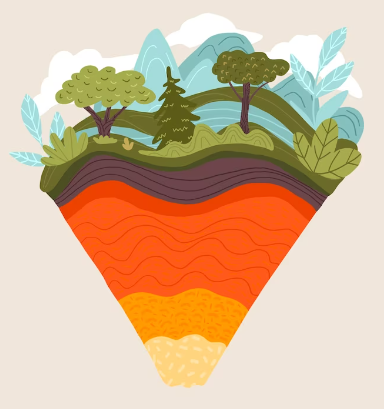
\includegraphics[width=2.58803in,height=2.75652in]{./imgs/img11.png}
\caption{Fonte: https://br.freepik.com/vetores-gratis/camadas-da-terra-desenhadas-a-mao-ilustradas\_18774832.htm\#query=camadas\%20da\%20terra\&position=44\&from\_view=search\&track=ais}
\end{figure}


\reduline{De cima para baixo: crosta, manto superior, manto inferior e núcleo.\hfill}
\linhas{1}

\num{9}  Lúcia e sua irmã mais nova, Lara, gostam de observar o céu pela noite.
  Em uma das observações Lara notou que a Lua havia mudado e questionou
  sua irmã mais velha: ``Por que conseguimos ver a lua de várias
  formas?''. Como você aconselharia Lúcia a explicar esse fenômeno para sua irmã?


\reduline{Lúcia deve explicar que vemos a Lua em diferentes fases devido à
luminosidade que recebe do Sol à medida que ela se desloca ao redor da Terra.\hfill}
\linhas{1}

\num{10}  Dentre todos os planetas do nosso Sistema Solar, pode-se dizer que a
  Terra tem uma característica especial, tendo em vista a vida que
  abriga. Descreva quais fatores tornaram possível a formação da vida na Terra.


\reduline{A Terra encontra-se em uma região chamada de habitável em nosso sistema
solar. Ou seja, ela recebe radiação solar suficiente para manter a
temperatura estável, permitindo a existência de água na forma líquida, essencial para a vida.\hfill}
\linhas{1}

\section{Treino}

\num{1} Observe a imagem a seguir e, com base nos seus conhecimentos, identifique quais são os planetas rochosos presentes no nosso sistema solar.

\begin{figure}[htpb!]
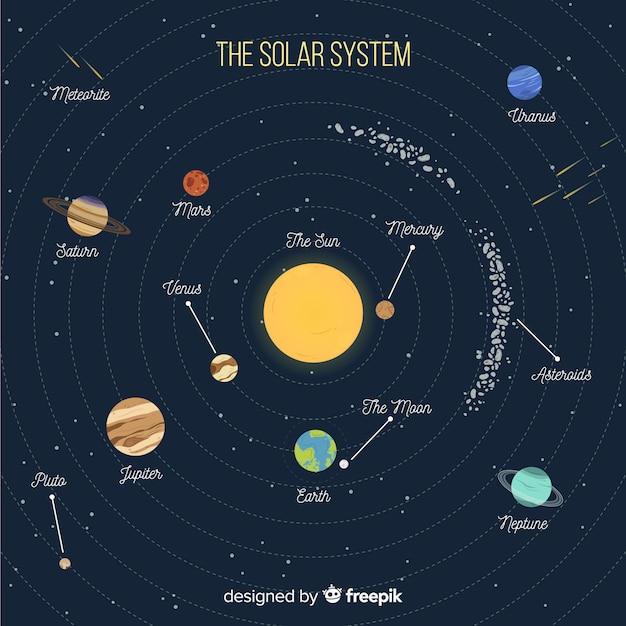
\includegraphics[width=2.89583in,height=2.89583in]{./imgs/img12.jpg}
%\caption{Esquema do Nosso Sistema Solar. Disponível em: https://br.freepik.com/vetores-gratis/esquema-do-sistema-solar-colorido-com-design-plano\_2826128.htm?query=planetas\%20do\%20sistema\%20solar\#from\_view=detail\_alsolike.}
\end{figure}

\begin{escolha}
\item
  Mercúrio, Vênus, Terra e Júpiter.
\item
  Netuno, Saturno, Terra e Urano.
\item
  Mercúrio, Vênus, Terra e Marte.
\item
  Saturno, Urano, Netuno e Plutão.
\end{escolha}

\num{2} Observe a imagem a seguir.

\begin{figure}[htpb!]

\includegraphics[width=2.77865in,height=2.63750in]{./imgs/img13.jpg}
%\caption{Novas fotos do James Webb podem revelar segredos sobre o nascimento de estrelas. CNN Brasil. 12/09/2022. Disponível em: https://www.cnnbrasil.com.br/tecnologia/novas-fotos-do-james-webb-podem-revelar-segredos-sobre-o-nascimento-de-estrelas/.}
\end{figure}

A imagem, registrada pelo Telescópio Espacial James Webb (NASA), mostra o
interior de uma nebulosa, onde nascem as estrelas. A partir dos seus
conhecimentos, justifique como é possível identificar o nascimento de
estrelas.

\begin{escolha}
\item
  Por meio da observação de elementos pesados e matéria escura.
\item
  Por meio da identificação de ferro na superfície da estrela.
\item
  Por meio da presença de grande quantidade de energia, gás e poeira cósmica.
\item
 Por meio da observação da Gigante vermelha em torno de uma nuvem de poeira.
\end{escolha}

\num{3}

\begin{quote}
Cientistas da Universidade da Califórnia-Riverside
(UCR) \textbf{simularam sistemas alternativos}~do nosso Sistema Solar,
descobrindo que se a órbita de Júpiter fosse mais achatada --- ou
"excêntrica" --- ela causaria grandes mudanças na órbita do nosso planeta. [...]
Se a órbita de Júpiter se tornasse mais excêntrica, a equipe
descobriu que a órbita da Terra seria empurrada para se tornar mais
excêntrica também. Isso significa que às vezes a Terra estaria ainda
mais perto do Sol do que já está. [...]
A equipe acha que seus resultados
podem ajudar os astrônomos a determinar quais planetas fora do Sistema
Solar -- exoplanetas -- poderiam ser habitáveis. [...]

\fonte{Sputinik Brasil. Mudança na órbita de Júpiter poderia tornar a Terra ainda mais favorável
à vida. Disponível em:
https://sputniknewsbrasil.com.br/20220914/mudanca-na-orbita-de-jupiter-poderia-tornar-a-terra-ainda-mais-favoravel-a-vida-24777610.html.
Acessado em: 20 fev. 2023.}
\end{quote}

Identifique, dentre as alternativas, aquela que descreve um importante
fator para a habitabilidade em um planeta.

\begin{escolha}
\item
  A distância de um planeta a sua estrela deve possibilitar temperaturas
  amenas e com baixas variações para que seja possível a existência de
  água líquida.
\item
  A órbita dos satélites naturais ao redor desse planeta deve ser a
  mesma órbita do planeta para que haja formação de água líquida.
\item
  O aumento da distância percorrida pelo planeta deve proporcionar
  aumento das regiões polares, evitando aquecimento do planeta.
\item
  A inclinação do planeta deve permitir que a radiação emitida por sua
  estrela seja a menor possível, pois radiação é algo nocivo.
\end{escolha}



